\documentclass[10pt,twocolumn]{elsart5p}
\usepackage{graphicx}
\usepackage{dcolumn}
\usepackage{amsmath}
\usepackage{amssymb}
\usepackage{bm}
\usepackage{natbib}
%\usepackage[noperiod]{jabbrv}
\usepackage{hyperref}

%
% Introduction
% ============
%
% Measures
% ========
% ISI        																	Done
% SPIKE      																	Done
% SPIKE-realtime      															Done
% SPIKE-future      																Done
% Edge effect																	Done
% Sampling   																	Done
% Representations      															Done
%
% SPIKY
% =====
% SPIKY-Intro   																	Done
% Structure     																	Done
% Input (data format), Spike Train Generator (Patterns, by hand)					Done 
% Output      																	Done
% Figure Layout      															Done
% GUI vs Loop      																Done
% Spike train surrogates (Significance), Comparison with Poisson					Done
% Comparison with other measures/implementations, Computational Cost (Memory, Speed)   Neb
%
% Discussion
% ==========
% Limitations
% Outlook
%

\begin{document}

\begin{frontmatter}

\title{SPIKY: A graphical user interface for monitoring spike train synchrony}

\author{Nebojsa Bozanic},
\ead{strance@gmail.com}
\author{Thomas Kreuz}
\ead{thomas.kreuz@cnr.it}


\address{Institute for complex systems, CNR, Sesto Fiorentino, Italy}


\date{\today}

\begin{abstract}

XXXXX Preliminary, to be edited in the end XXXXX
Recently, the SPIKE-distance has been proposed as a measure of spike train synchrony which is both parameter-free and time-scale independent. Since it relies on instantaneous estimates of spike train dissimilarity, it is also time-resolved which makes it possible to track changes in instantaneous clustering, i.e., time-localized patterns of (dis)similarity among multiple spike trains. Further features include selective and triggered temporal averaging as well as the instantaneous comparison of spike train groups. Besides the regular SPIKE-distance, there also exists a causal variant which is defined such that the instantaneous values of dissimilarity rely on past information only so that time-resolved spike train synchrony can be estimated in real-time. Finally, here we introduce the future SPIKE-distance which can be used in triggered temporal averaging in order to evaluate the effect of certain spikes or of certain stimuli features on future spiking. In the first part of this report we address some of the computational aspects in the calculation and implementation of the SPIKE-distance while in the second part we present SPIKY, a graphical user interface which facilitates the application of the SPIKE-distance and all its variants to both simulated and real data.
 
\end{abstract}


%\begin{keyword}
%    time series analysis; spike trains; clustering; neuronal coding; SPIKE-distance; ISI-distance; graphical user interface; Matlab; SPIKY
%\end{keyword}

\end{frontmatter}

\newcommand{\abb}{\small\sf}

%
%
% *************************************************************************************
% ******************************************************** Introduction ***************
% *************************************************************************************
%
%
\section{\label{s:Intro} Introduction}

Spike train distances are measures that when applied to a set of spike trains yield low (high) values for very similar (dissimilar) spike trains. Essentially there are two major scenarios for using spike train distances to estimate the degree of synchrony between two or more spike trains. The most common scenario is the simultaneous recording of a neuronal population, typically in some kind of spatial multi-channel setup. If different neurons emit spikes simultaneously, these spikes are "synchronous" in the classical sense of the word, which is derived from Greek and describes events "occurring at the same time" \citep{Pikovsky01}. Synchronization between individual neurons has been proven to be of high prevalence in many different neuronal circuits. Examples include the visual cortex \citep{Tiesinga08} and the retina \citep{Shlens08} for which numbers of spike coincidences considerably above chance level have been reported. As of now many open questions remain regarding the spatial scale and the nature of interactions (e.g., pairwise or higher order, see \citep{Nirenberg07}) as well as their functional significance for neuronal coding and information processing \citep{Kumar10}.

In the other major scenario the neuronal spiking response is recorded in different time intervals. In order to allow a meaningful confrontation there has to be a temporal reference point which is typically set by some kind of trigger (e.g., the onset of an external stimulation). There are two prominent applications for this successive trials scenario. The first one is to test for the reliability of individual neurons by presenting the same stimulus repeatedly (e.g., \citet{Mainen95}). In contrast, when different stimuli are used one is mostly interested in the features of the response that provide the optimal discrimination since this might allow drawing conclusions regarding the nature of the neuronal coding (e.g., \citet{Victor05}). These two applications are related since for a good clustering performance one needs not only a pronounced discrimination between stimuli (high inter-stimulus spike train distances) but also a high reliability for the same stimulus (low intra-stimulus spike train distances).

In both population and successive trial recordings a high temporal resolution would be very desirable. Analyzing the changing spiking patterns of large ensembles of single neurons in epilepsy patients could lead to a better understanding of the mechanisms of seizure generation, propagation, and termination \citep{Truccolo11, Bower12} in the same way as the analysis of neuronal responses to successive presentations of time-dependent stimuli could help to understand the role of synchronous firing in neuronal coding \citep{Miller08}. Moreover, in population recordings it would be even more advantageous to be able to monitor spike train synchrony in realtime. In epilepsy this would be a necessary condition for the implementation of a prospective seizure prediction algorithm \citep{Mormann07}, but it could also be very useful for the rapid online decoding of neural signals needed to control prosthetics \citep{Hochberg06, Sanchez08}.


multivariate extension of event synchronization


Many different representations, i.e. degrees of information reduction


Need for a graphical user interface (GUI)

Another advantage of having a graphical user interface is the easy accessibility to users that are not familiar with programming environments such as Matlab.

Improvements regarding the possible size of the dataset (memory and speed)

edge effect

Computational aspects

The remainder of this paper is organized as follows. We start with an overview of the different levels of information reduction for the time-resolved measures in Section \ref{ss:Information-reduction}. These range from the most detailed representation in which one instantaneous value is obtained for each pair of spike trains to the most condensed representation in which successive temporal and spatial averaging leads to one single distance value which describes the overall level of synchrony for a group of spike trains over a given time interval.

SPIKY, our graphical user interface (GUI) for monitoring spike train synchrony, is presented in Section \ref{s:SPIKY}. In Subsection \ref{ss:Access} explain how to get access to the codes and the large library of documentation (which includes text files, images, movies, as well as screen recordings with voice-over in which the user is guided step by step through some of the most important features of SPIKY). Subsequently, in Subsection \ref{ss:Structure} we introduce the structure and the workflow of the program. We show how to input spike train data, how to change the layout of the figures and how to export results. We also present two programs included in the SPIKY-package which are complementary to the graphical user interface itself. While the program 'SPIKY\_loop' (Subsection \ref{ss:GUI-vs-loop}) is meant to be used for the collective analysis of many different datasets (e.g. when the statistics of a certain quantity should be evaluated over all available datasets), the program 'SPIKY\_loop\_surro' (Subsection \ref{ss:Spike-train-surrogates}) was designed to evaluate the statistical significance of the results obtained for the original dataset by comparing them against the results obtained for spike train surrogates generated from that dataset. In Subsection \ref{ss:Comparison} we investigate the performance of our new implementation of the time-resolved measures of spike train synchrony and compare it with previously published codes (e.g. \citet{Rusu14}). In Section \ref{s:Discussion} we summarize both the methods and the program, discuss their limitations and present an outlook on future developments.

Finally, in the appendix we introduce and discuss the different measures available in SPIKY. These include event synchronization (Section \ref{App-s:Event-Synchronization}), the ISI-distance and the SPIKE-distance (as well as its realtime and future variants). In Subsection \ref{ss:Improvements} we present the improvements we have realized in this new implementation of the measures such as the correction of the edge-effect and the increase of memory efficiency by avoiding sampling. 

%
%
% *************************************************************************************
% ********************************************************** Measures *****************
% *************************************************************************************
%
%
	


\section{\label{s:Information-reduction} Levels of information reduction}

The ISI- and the SPIKE-distance combine a variety of properties that make them well suited for applications to real data. In particular, they are conceptually simple, computationally efficient, and easy to visualize in a time-resolved manner. By taking into account only the preceding and the following spike in each spike train, these distances rely on local information only. They are also time-scale-adaptive since the information used is not contained within a window of fixed size but rather within a time frame whose size depends on the local rate of each spike train.

Moreover, the sensitivity to spike timing and the instantaneous reliability achieved by the SPIKE-distance opens up many new possibilities in multi-neuron spike train analysis \citep{Kreuz13}. These build upon the fact that there are several levels of information reduction all of which we describe in the following. As illustration we use the detailed analysis of an artificially generated spike train dataset (see upper subplot of Fig. \ref{fig:Fig2-SPIKE-Representations}A for the rasterplot). 
%
% #########################################################################################
% #########################################################################################
% #################################################### Figure 2 ###########################
% #########################################################################################
% #########################################################################################
%
\begin{figure}
    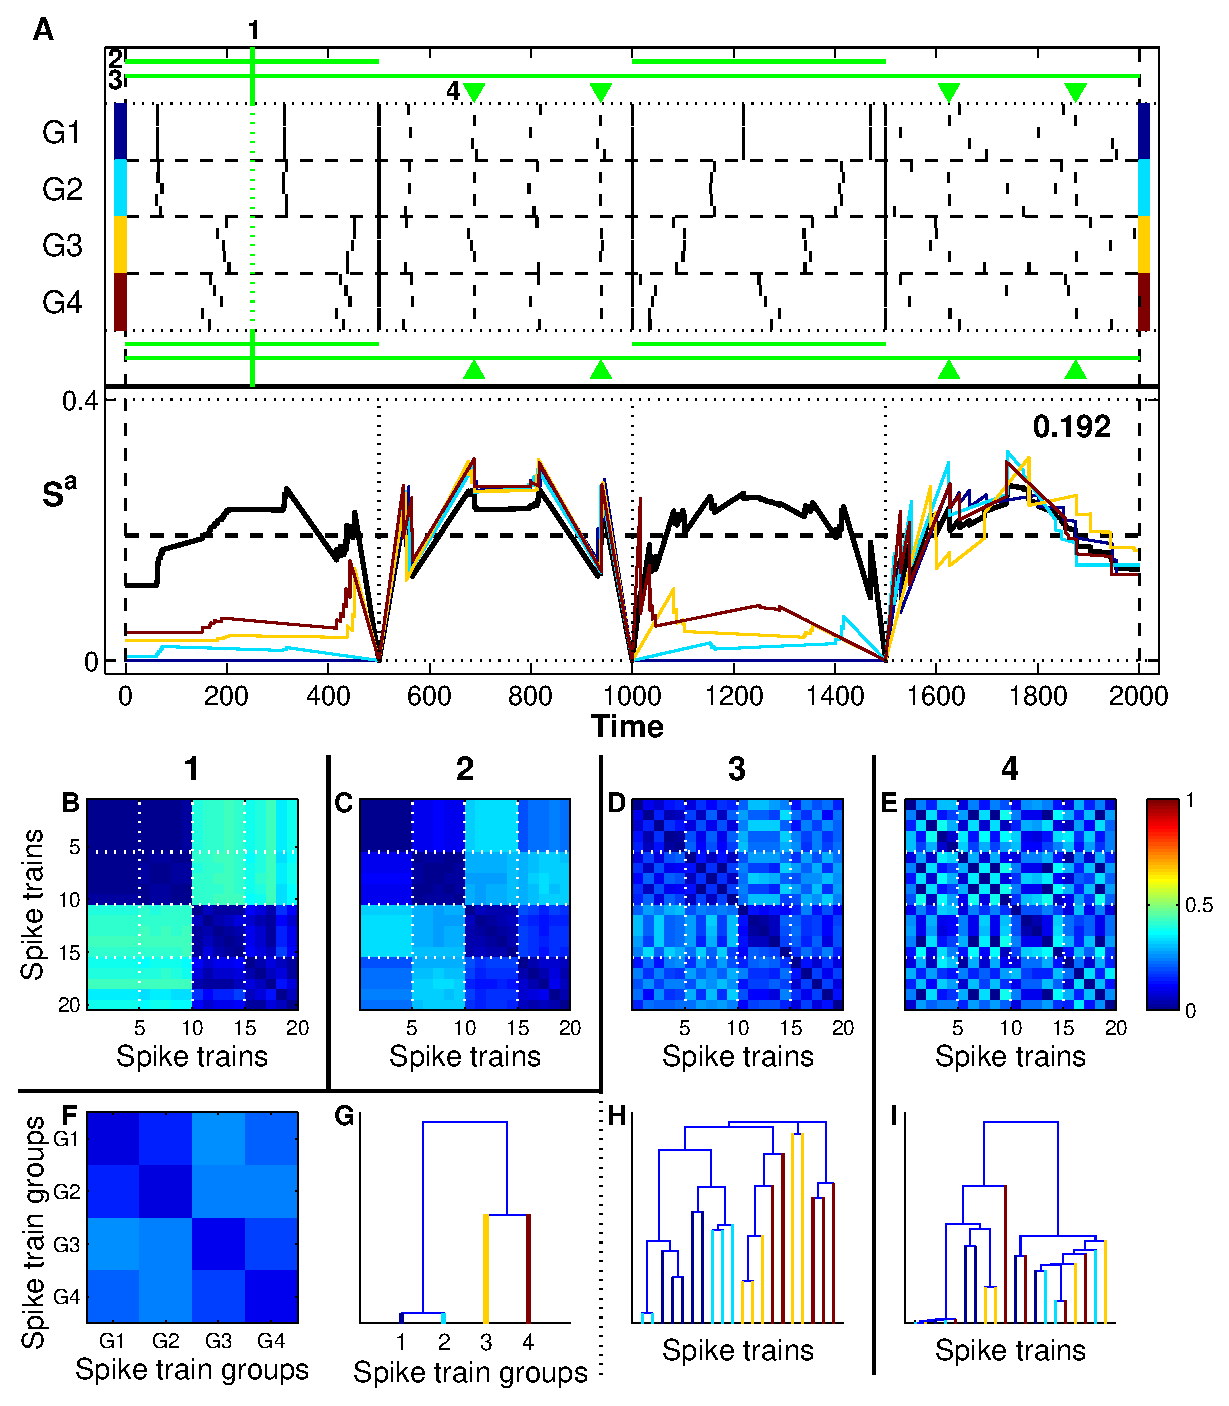
\includegraphics[width=85mm]{Fig2_SPIKE_Representations.eps}
    \caption{\abb\label{fig:Fig2-SPIKE-Representations} The different levels of information reduction for the SPIKE-distance.  A. Top: Spike rasterplot of $20$ artificially generated spike trains divided in $4$ spike train groups of $5$ spike trains each. The clustering behavior changes every $500$ ms. Bottom: Dissimilarity profiles of the SPIKE-distance for the four spike train groups (thin color-coded lines) and for all spike trains (thick black line). The overall dissimilarity is defined as the temporal average of the dissimilarity profile of all spike trains ($0.192$ in this case) and is marked by a black horizontal line.  B-E. Matrices of pairwise instantaneous dissimilarity values for a single time instant, for two selective averages and for a triggered average.  F. Matrices of overall pairwise instantaneous dissimilarity values for the $4$ spike train groups.  G. Dendrogram of spike train group matrix in F.  H-I. Dendrogram of spike train matrices in D and E. Note that the triggered averages in contrast to the overall average captures the local similarity between $5$ of the spike trains.}
\end{figure}
%
% #########################################################################################
% #########################################################################################
% #################################################### Figure 2 ###########################
% #########################################################################################
% #########################################################################################

\subsection{\label{ss:Full-matrix-and-cross-sections} Full matrix and cross sections}

The starting point is the most detailed representation in which one instantaneous value is obtained for each pair of spike trains (see Eq. \ref{eq:Bi-Spike-Diss-Improved}). This representation could be viewed as a movie of a symmetric pairwise dissimilarity matrix in which each frame corresponds to one time instant (an example can be found in the supplementary material of \citep{Kreuz13}). For a movie of finite length the time axis necessarily has to be sampled but in principle this most detailed representation is continuous and consists of an infinite number of values. However, since all dissimilarity profiles are piecewise linear (with potential discontinuities only at the times of the spikes) there is a lot of redundancy. Using the most compact and memory-efficient representation one can store all pairwise dissimilarity profiles in a matrix of size 'number of unique spikes in the pooled spike train' $\times$ 'number of spike train pairs' ($\times 2$ for the SPIKE-distance, see Section \ref{sss:Sampling}).

From this matrix, it is possible to extract any desired information. By selecting a pair of spike trains, one obtains the bivariate dissimilarity profile $S (t)$ for this pair of spike trains. Selecting a time instant $t_s$ (and using linear interpolation for time instants in between spikes) yields an instantaneous matrix of pairwise spike train dissimilarities $S_{mn}(t_s)$. This matrix can be used to divide the spike trains into instantaneous clusters, that is, groups of spike trains with low intra-group and high inter-group dissimilarity.

\subsection{\label{ss:Spatial-and-temporal-Averaging} Spatial and temporal averaging}

Another way to reduce the information of the dissimilarity matrix is averaging. There are two possibilities that commute: the spatial average over spike train pairs and the temporal average.

The local average over spike train pairs yields a dissimilarity profile for the whole population. Temporal averaging over certain (continuous or noncontinuous) intervals on the other hand leads to a bivariate distance matrix (in real data, these intervals could be chosen to correspond to different external conditions such as normal vs. pathological, asleep vs. awake, target vs. non-target stimulus, or presence/absence of a certain channel blocker). Finally, in both cases, application of the respective remaining average results in one distance value that describes the overall level of synchrony for a group of spike trains over a given time interval.

\subsection{\label{ss:Triggered-Averaging} Triggered averaging}

The fact that there are no limits to the temporal resolution allows further analyses such as internally or externally triggered temporal averaging. Here, the matrices are averaged over certain trigger time instants only. The idea is to check whether this triggered temporal average is significantly different from the global average since this would indicate that something peculiar is happening at these trigger instants. The trigger times can either be obtained from external influences (such as the occurrence of certain features in a stimulus) or from internal conditions (such as the spike times of a certain spike train). External triggering is a standard tool to address questions of neuronal coding, for example, it can be used to evaluate the influence of localized stimulus features on the reliability of neurons under repeated stimulation. In multi-neuron data, internal triggering might help to uncover the connectivity in neural networks or to detect converging or diverging patterns of firing propagation. An example is shown in Fig. \ref{fig:Fig2-SPIKE-Representations}E. Here, neurons $2$, $9$, $14$, and $19$ follow the $7$-th neuron during the 2nd and the 4th subinterval. This can be revealed by triggering on the spike times of neuron $7$ during these sub

A last possibility is spatial averaging such that the spike trains are manually assigned to subgroups, and a block matrix (and the corresponding dendrogram XXXXX) is obtained by averaging over the respective submatrices of the original dissimilarity matrix. An example is shown in Fig. \ref{fig:Fig2-SPIKE-Representations}F and the corresponding dendrogram is depicted in Fig. \ref{fig:Fig2-SPIKE-Representations}G. In applications to real data, these groups could be different neuronal populations or responses to different stimuli, depending on whether the spike trains were recorded simultaneously or successively.

XXXX Create one Matlab figure which includes as many representations as possible XXXXX

%
%
% *************************************************************************************
% **************************************************************** SPIKY **************
% *************************************************************************************
%
%
\section{\label{s:SPIKY} SPIKY}

SPIKY is a graphical user interface (GUI) for monitoring synchrony between artificially simulated or experimentally recorded neuronal spike trains. It is an implementation of the ISI- and the SPIKE-distance (including simulations of its realtime and future variants) which allows  interactive access to all the different representations described in Section \ref{s:Information-reduction}. SPIKY is a free software package programmed by Thomas Kreuz and Nebojsa Bozanic. All source codes are written in Matlab (MathWorks Inc, Natick, MA, USA) with the most time-consuming loops coded in MEX-files \footnote{In our case these are subroutines written in C. However, as some users may not have access to a suitable C compiler, SPIKY contains the (slower) pure Matlab code as well.}. SPIKY is not stand-alone but requires Matlab to run. XXXXX Update, now stand-alone? XXXXX.


\subsection{\label{ss:Access} Access to SPIKY and how to get started}

SPIKY is distributed under a BSD licence (Copyright (c) 2014, Thomas Kreuz, Nebojsa Bozanic. All rights reserved.). A zip-package containing all the necessary files can be accessed for free on the \href{http://www.fi.isc.cnr.it/users/thomas.kreuz/Source-Code/SPIKY.html}{download page} (\url{http://www.fi.isc.cnr.it/users/thomas.kreuz/Source-Code/SPIKY.html}). This package also contains a folder with lots of documentation (such as a FAQ-file and an introduction to all individual elements and all individual files of SPIKY). Further information and many demonstrations (both images and movies) can be found on the download page and on the \href{https://www.facebook.com/SPIKYgui}{SPIKY Facebook-page} (\url{https://www.facebook.com/SPIKYgui}). Both of these pages are used to announce updates and distribute the latest information about new features. They also provide the user with an opportunity to provide feedback and ask questions.

The Facebook-page include various screen recordings with voice-over in which the user is guided step by step through some of the most important features of SPIKY. All of these movies can also be viewed on the \href{https://www.youtube.com/channel/UCgSz0YQ5lWdVF0_Z1FNN0Bw}{SPIKY Youtube-channel} (\url{https://www.youtube.com/channel/UCgSz0YQ5lWdVF0_Z1FNN0Bw}).

After having downloaded SPIKY from the download page the user has to first extract the zip-package which leaves all files in one folder named 'SPIKY'. If the system has a suitable MEX-compiler installed, the MEX-files can be compiled from within this folder by running the m-file 'SPIKY\_compile\_MEX'. The last step is to run the m-file 'SPIKY'. XXXXX Stand-alone version? XXXXX 

When SPIKY is running, the user can find quick information about the individual elements of the graphical user interface by activating the 'Hints'-checkbox in the 'Options'-Menu. Hovering with the mouse cursor above the elements of interest will then show short hints. An overview of all the information contained in the hints can be found in the documentation file 'SPIKY-Elements.doc'. Furthermore, at each step the suggested element for the next user action is highlighted by a bold font. 

To get the user started quickly, SPIKY provides a few (artificial) example datasets from previous publications. The most useful example is the entry 'Clustering' in the 'Selection: Data'-listbox. This dataset has already been used in several figures as well as in the supplementary movie of \cite{Kreuz13}. A good introduction to SPIKY would be to follow this example through till the end advancing from panel to panel by pressing the highlighted button. In a second step one could reset and run the same example again while changing some parameters in order to see the consequences. Note that it is not necessary to set all the parameters each time when SPIKY is started. Rather it is possible to use the file 'SPIKY\_f\_user\_interface' to set and modify the spike train data as well as the parameters (again refer to the dataset 'Clustering' for an example).


\subsection{\label{ss:Structure} Structure and workflow of SPIKY}

Overall, SPIKY has a rather linear workflow, however, it is much more interactive than previous implementations of the ISI- and the SPIKE-distance and there are many potential shortcuts and loops along the way. As you can see in the SPIKY-flowchart in Fig. \ref{fig:Fig3-SPIKY-Flowchart}, the general flow is clearly directed from the input of spike train data to the output of results. So the first step the user has to do is to give SPIKY spike train data (i.e. sequences of spike times) to work with. There are three possibilities to do so: one can make use of predefined examples, load data from a file, or employ the spike train generator (see Section \ref{sss:Input} for more details).
%
% #########################################################################################
% ######################################################################################### #################################################### Figure 3 ###########################
% #########################################################################################
% #########################################################################################
%
\begin{figure}
    \includegraphics[width=85mm]{Fig3_SPIKY_Flowchart.eps}
    \caption{\abb\label{fig:Fig3-SPIKY-Flowchart} Flowchart describing the workflow of SPIKY from 	the input of spike train data to the output of results. A typical SPIKY-session begins at the top with 'Get data', then goes clockwise and ends on the left with 'Get results'. In the center of the circle the SPIKY-logo is depicted.}
\end{figure}
%
% #########################################################################################
% #########################################################################################
% #################################################### Figure 3 ###########################
% #########################################################################################
% #########################################################################################

Once the full dataset is there, modification is still possible. One can restrict the analysis to a specific subset, e.g., select a smaller time window and/or a subset of spike trains. It is also possible to impose some external structure on the rasterplot (spike trains vs time). SPIKY allows the definition of two types of spike train separators (e.g. neurons from the left vs. neurons from the right hemisphere) and two types of time markers (e.g. specific events such as seizure onset and offset in epilepsy, trigger onset during stimulation etc.). It also enables the user to define spike train groups. Depending on the setup these could be spike trains recorded in different brain regions or upon presentation of different kinds of stimuli. Fig. \ref{fig:Fig4_Movie_Screenshot} shows an example of a raster plot with annotations marking all these different elements.
%
% #########################################################################################
% #########################################################################################
% #################################################### Figure 4 ###########################
% #########################################################################################
% #########################################################################################
%
\begin{figure}
    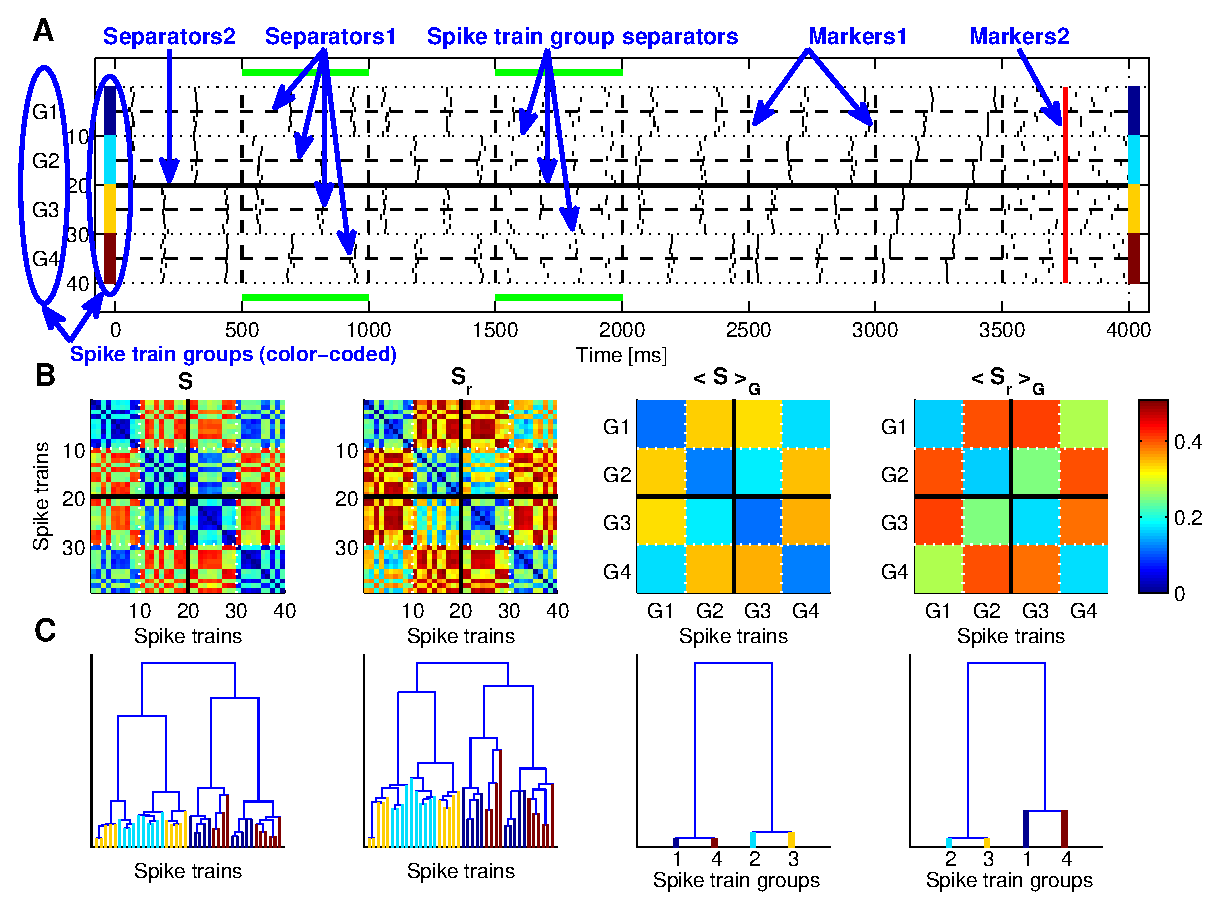
\includegraphics[width=85mm]{Fig4_Movie_Screenshot.eps}
    \caption{\abb\label{fig:Fig4-Movie-Screenshot} Annotated screenshot from a movie.   A.				Artificially generated spike trains.   B. Dissimilarity matrices obtained by averaging 			over two separate time intervals for both the regular and the real-time SPIKE-distance 			as well as their averages over subgroups of spike trains (denoted by $<\cdot>_G$).   C. 				Corresponding dendrograms.}
\end{figure}
%
% #########################################################################################
% #########################################################################################
% #################################################### Figure 4 ###########################
% #########################################################################################
% #########################################################################################

After updating all of these data parameters the next step is to select the measures to be calculated. In addition to the measures described in Section \ref{s:Measures} we also include the Peri-Stimulus Time Histogram (PSTH) as a time-resolved standard approach widely used in spike train analysis. However, note that the PSTH is a complementary approach which describes overall firing rate and (to some precision) timing. It is not a measure of spike train synchrony \citep{Kreuz11} since it is invariant to shuffling spikes among the spike trains yielding the same value regardless of how spikes are distributed among the different spike trains. At the same time the user can select successive frames for a temporal analysis of spike train patterns. These can be individual time instants for cross sections, temporal intervals for selective averages and sequences of time instants for triggered averages (see Section \ref{s:Information-reduction}).

Now the actual calculation of the measures takes place. For reasonably sized datasets this should take at most a few seconds. Larger datasets are divided in smaller subintervals and the calculation will be performed in a loop which might take longer (cf. Section \ref{ss:Limitations}). It is at this point that SPIKY becomes truly interactive. Now the user can switch between different representations of the results (such as dissimilarity profiles, dissimilarity matrices and dendrograms). Regarding matrices and dendrograms one can decide whether one wants to compare different representations or look at them in sequence.

The presentation can be restricted to smaller time windows and/or subsets of spike train, and temporal and spatial averaging (for example moving average and average over spike train groups) can be performed. It is possible to add further figure elements such as spike number histograms, overall averages, or dissimilarity profiles for individual spike train groups. At this stage the user can also retrospectively change the appearance of all the individual elements of the figure (see Section \ref{sss:Figure-Layout} for more details). Finally, SPIKY allows to extract both data and results to the Matlab workspace for further analysis, and it is also possible to save individual figures as postscript-file or a sequence of images as an 'avi'-movie (for more details see Section \ref{sss:Output}).


\subsubsection{\label{sss:Input} Input}

There are three different possibilities to input spike train data into SPIKY.

The first option is to select one of the predefined examples which are generated using Matlab-code. Initially these are the examples used in \citep{Kreuz13} but one can also define new examples.

The second option is to load spike train data from a file. Two different file formats are allowed, '.mat' and '.txt' (ASCII) files. For the mat-files SPIKY currently allows three different kinds of input formats (further formats can be added on demand).

\begin{itemize}
\item cell arrays (ca) with just the spike times. This is the preferred format used by SPIKY since it is most memory efficient. The two other formats will internally be converted into this format.
\item regular matrices with each row being a spike train and zero padding (zp) in case the spike numbers are different.
\item matrices representing time bins where each zero/one (01) indicates the absence/presence of a spike
\end{itemize}

If case of a mat-file SPIKY looks for a variable called 'spikes', if it cannot find it you have the chance to select the variable name (or field name) which contains the spikes via an input mask which provides a hierarchical structure tree of the variable structure. In the text format spike times should be written as a matrix with each row being one spike train. The SPIKY-package contains one example file for all four formats ('testdata\_ca.mat', 'testdata\_zp.mat', 'testdata\_01.mat' and 'testdata.txt').

The third option is to create new spike train data via the spike train generator. After setting some defining variables (number of spike trains, start and end time, sampling interval) you can build your spike trains by using predefined spike train patterns (such as periodic, splay, uniform or Poisson) and/or by manually adding, shifting and deleting individual spikes or groups of spikes.


\subsubsection{\label{sss:Figure-Layout} Figure-Layout}

SPIKY was designed in a way that allows to directly generate figures suitable for publication. To this aim the user is given control over the appearance of every individual element (e.g. fonts, lines etc.) in each type of figure. There are two ways to determine essential properties such as color, font size or line width. Most conveniently, one can use the file 'SPIKY\_f\_user\_interface' to define the standard values for all the parameters that describe the principal layout of the figure. But it is also possible to change elements in the active figure while the program is already running. To do so the user has to simply click the right mouse button on the element to be changed. A context menu will appear which lets the user either edit either the properties of individual elements or of all elements of a certain type. This also includes the string property of any font (title, x- and y-labels etc.).

If a figure contains more than one subplot (besides the combined subplot containing the spike rasterplot and dissimilarity profiles these are typically subplots with dissimilarity matrices and dendrograms), it is also possible to change their position and size. To do so just move the cursor to the respective axis (either just left or just below the subplot) and click the right mouse button. Now one can edit all position variables by hand or change the x-position, the y-position, the width and the height individually. In case there are several dissimilarity matrices / dendrograms one can do this either for an individual matrix / dendrogram or for all of them at the same time.


\subsubsection{\label{sss:Output} Output}

From within SPIKY it is possible to extract the spike trains and the results of the analyses (measure profiles, matrices, dendrograms) to the Matlab workspace for further processing. When one clicks the right mouse button on the element whose data one wishes to extract results will be stored in variables such as 'SPIKY\_spikes', 'SPIKY\_profile\_X\_1', 'SPIKY\_profile\_Y\_1', 'SPIKY\_profile\_name\_1' as well as 'SPIKY\_matrix\_1' and 'SPIKY\_matrix\_name\_1'. In addition, the results obtained during an analysis will automatically be stored in the output structure 'SPIKY\_results' which will have one field for each measure selected. Depending on the parameter selection within SPIKY, for each measure the structure can contains the following subfields which largely correspond to the different representations identified in Section \ref{s:Information-reduction}:

\begin{itemize}
\item SPIKY\_results.$<$Measure$>$.name: Name of selected measures (helps to identify the order within all other variables)
\item SPIKY\_results.$<$Measure$>$.distance: Level of dissimilarity over all spike trains and the whole interval. This is just one value, obtained by averaging over both spike trains and time
\item SPIKY\_results.$<$Measure$>$.matrix: Pairwise distance matrices, obtained by averaging over time
\item SPIKY\_results.$<$Measure$>$.x: Time-values of overall dissimilarity profile
\item SPIKY\_results.$<$Measure$>$.y: Overall dissimilarity profile obtained by averaging over spike train pairs
\end{itemize}

Note that the dissimilarity profiles are not equidistantly sampled. Rather they are stored as memory-efficiently as possible which means just one value for each interval of the pooled spike train for the ISI- and two values for the SPIKE-distance. Since this format can be more difficult to process, the functions 'SPIKY\_f\_selective\_averaging', 'SPIKY\_f\_triggered\_averaging', and 'SPIKY\_f\_average\_pi' are provided in order to compute the selective average over time intervals, the triggered over time instants, or the average over many dissimilarity profiles, respectively. Furthermore, for the ISI-distance the function 'SPIKY\_f\_pico.m' can be used to obtain the average value as well as the x- and y-vectors for plotting.

Besides the standard way to work with Matlab-figures SPIKY also offers the opportunity to save each figure as a postscript-file. Finally, it is possible to save a sequence of images as an 'avi'-movie.


\subsection{\label{ss:GUI-vs-loop} GUI vs. loop}

SPIKY was mainly designed to facilitate the detailed analysis of one dataset. It enables the user to switch between different representations (see Section \ref{s:Information-reduction}) and to zoom in on both spatial and temporal features of interest. However, SPIKY is not very suitable for the collective analysis of many different datasets when e.g. the statistics of a certain quantity such as an average over certain time intervals should be evaluated over all available datasets in some kind of loop. For these purposes the SPIKY-package contains a program called 'SPIKY\_loop' which is complementary to SPIKY. It is not a graphical user interface but it should be simple enough (and plenty of examples are provided) to allow everyone to run the same kind of analysis for many different datasets and to evaluate and compare their 'SPIKY\_results'. 'SPIKY\_loop' uses the full functionality of SPIKY such as access to time instants, selective and triggered averages as well as averages over spike train groups.

So combining these two programs it is possible to first use SPIKY for a rather exploratory but detailed analysis of a limited number of individual datasets and then use SPIKY\_loop and its output structure 'SPIKY\_loop\_results' to verify whether any effect discovered on the example dataset is consistently present within all of the datasets.


\subsection{\label{ss:Spike-train-surrogates} Spike train surrogates and significance}

An important question that has not yet been asked is the one of statistical significance. Given a certain value of the SPIKE-distance how can one judge whether it reflects a significant decrease or increase in spike train synchrony and does not just lie within the range of values obtained for random fluctuations. One way to address this question is the use of spike train surrogates \citep{Kass05, Gruen09, Louis10}. The idea is to compare the results obtained for the original dataset versus the results obtained for spike train surrogates generated from that dataset. If the value obtained for the original lies outside the range of values for the surrogates this value can be assumed to be significant to a level defined by the number of surrogates used (e.g. $\alpha = 0.05$ for $19$ surrogates or $\alpha = 0.001$ for $999$ surrogates).

%The SPIKY-package contains a program 'Spiky\_loop\_surro' which was designed to look at significance.So far it includes four different types of spike train surrogates. They differ in the properties that are preserved %and maintain either the individual spike numbers (obtained by shuffling the spikes), the individual interspike %interval distribution (obtained by shuffling the interspike intervals), the pooled spike train (obtained by %shuffling spikes among the spike trains) or the peri-stimulus time histogram (PSTH) (obtained by drawing from the %probability density function (PDF) of the data).

The SPIKY-package contains a program `SPIKY\_loop\_surro' which was designed to look at significance. So far it includes four different types of spike train surrogates. They differ in the properties that are preserved and maintain either the individual spike numbers (obtained by shuffling the spikes), the individual interspike interval distribution (obtained by shuffling the interspike intervals), the pooled spike train (obtained by shuffling spikes among the spike trains) or the distribution using a general method for resampling from a given distribution using {\it the inverse transformation method} which is based on having a uniform (0, 1) random variable $U$, where for any distribution function $F$ if there is a defined random variable $X$ such that $X = F^{-1}(U)$ then the random variable $X$ has a distribution function $F$. [$F-'(u)$ is defined to equal that value $x$ for which $F(x) = u.$]



% Daniel's Email 13.07.2011:
%
% Regarding the use of Poisson processes to have a benchmark it will have different implications depending on the structure of your data. If the rate is almost constant then comparing to processes with the same estimated average rate is the best option. If the rate is time-dependent you may want to compare with processes which are Poisson but mimic the same time-dependent profile of the rate. These are just alternatives that give you complementary information on the structure of the reliability.
% Surrogate data with the same time dependent rate can be obtained by randomly reassigning each spike to any of the spike trains.


\subsection{\label{ss:Comparison} Comparison with other implementations}

Python-Implementation of SPIKE-distance courtesy of Jeremy Fix:

\url{http://jeremy.fix.free.fr/Softwares/spike.html}

Python-Implementation of the pairwise ISI-distance courtesy of Michael Chary:

\url{https://pypi.python.org/pypi/ISIpy/1.0.1}

R{\v a}zvan Florian:

\url{https://github.com/modulus-metric/spike-train-metrics}

\citep{Rusu14}

While all of these previous implementations are restricted to the overall dissimilarity profile and its temporal average (the overall dissimilarity), SPIKY also allows the user to interactively access all of the many different levels of information reduction introduced in Section \ref{s:Information-reduction}.




HRLAnalysis$^{TM}$ \citep{Thibeault14}

XXX Nebojsa figure (Performance comparison) XXX
%
%\begin{figure}
%    \includegraphics[width=85mm]{FigXX_Performance_Comparison.eps}
%    \caption{\abb\label{fig:FigXX-Performance-Comparison} XXX Add correct figure XXX Performance comparison: Time %needed for computing various distances, as a function of the number of spikes in the spike trains. For the ISI- and %the SPIKE-distance we show the curves for both the old (sampling-based) and the new algorithm.}
%\end{figure}

\subsection{\label{ss:Comparison} Comparison with other implementations}

Matlab provides a powerful toolbox for processing vectorized data because of the high level parallelization, while its GUI has engaging visualization capabilities. Some possible problems in using Matlab for processing spike train data could relate to the fact that interpreted language are slow. Addressing this issue, we converted the most time consuming functions to C. Under Matlab (2007b), we observed a significant speed up of functions written in C  with respect to the ones written in Matlab. 

C functions do not only lead to an increase in performance, they can also easily be incorporated into other programming platforms (such as Python).

% One of the disadvantages of using Matlab while processing large spike trains is that Matlab casts all floating-point numbers to 64-bit double precision by default, thus using large amounts of memory to handle large datasets, partially this problem can be solved converting to 32-bit single precision, which has been successfully issued in SPIKY. 

%Current version of SPIKY focuses on handling of large spike trains, dividing input spike times into groups yet still allowing usage of massive parallelization.

%There was a considerable effort to bring performance along with usability, so SPIKY may have a higher than expected level of specificity. The variety of options included may be discouraging to potential users.

For the sake of an unbiased comparison all algorithms have been implemented in C++, Visual C++ 12.0, and the complete source codes are available on http://wwwold.fi.isc.cnr.it/users/thomas.kreuz/ XXXXX to upload XXXXX. The following results have been achieved on an Intel Core i7-4700MQ CPU @ 2.4 GHz.

\begin{figure}
    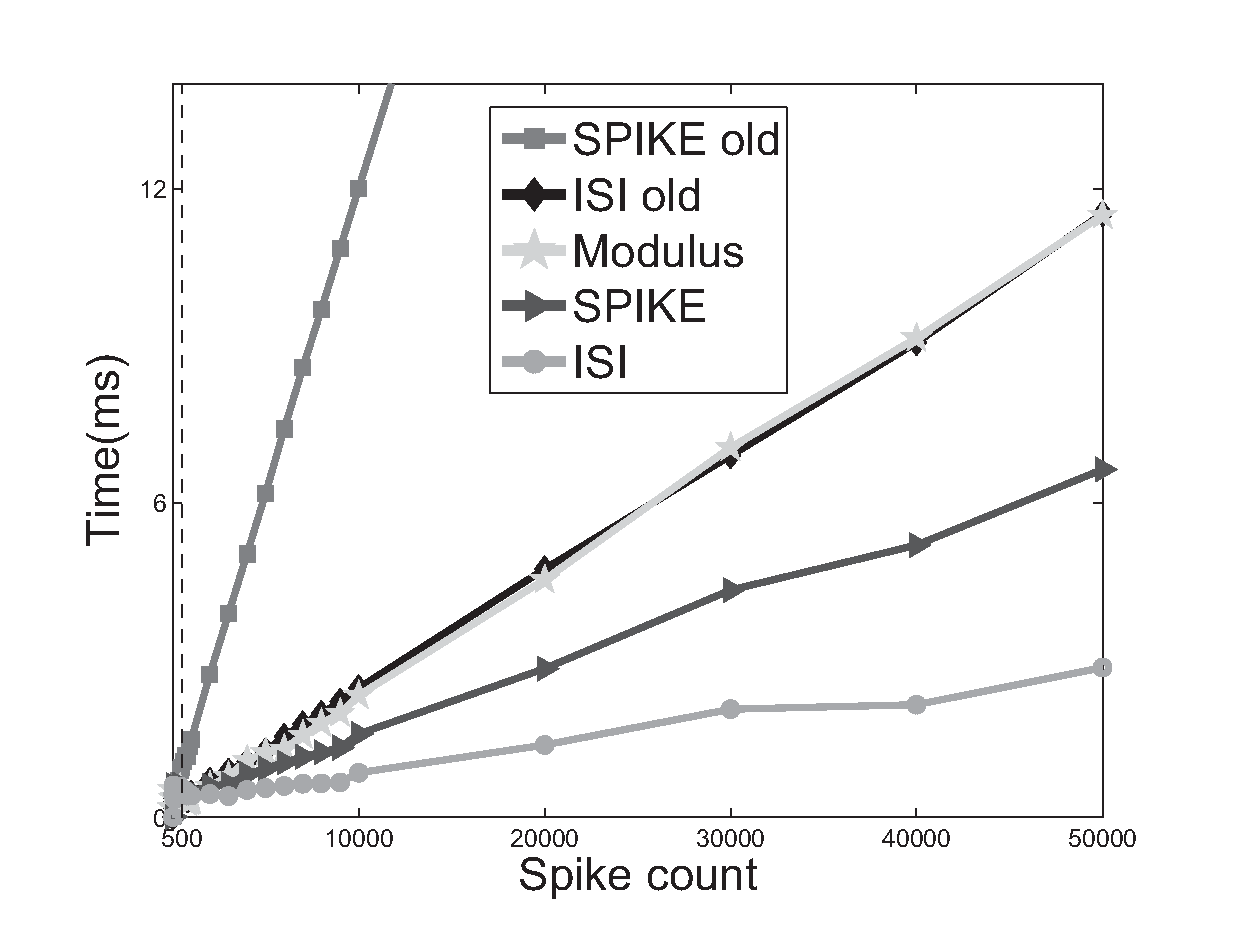
\includegraphics[width=85mm]{Fig5_Performance_Comparison.eps}
    \caption{\abb\label{fig:Fig5-Performance-Comparison} Performance comparison: Time needed for computing various distances, as a function of the number of spikes in the spike trains. For the ISI- and the SPIKE-distance we show the curves for both the old (sampling-based) and the new algorithm.}
\end{figure}

In order to show how different implementation of the same method can have different complexity classes, previous implementations for ISI-distance, SPIKE-distance and modulus metric are taken and compared versus novel ones (Figure 5).

The setup for the comparison was taken from XXX(cite{rusu})XXXX. Algorithms were tested using simulated spike trains. As spike train input we used random processes with different numbers of spikes. Figure \ref{fig:Fig5-Performance-Comparison} shows average time needed to compute distances as a function of number of spikes. The results were averaged over 10,000 trials. The simulations confirmed that the new 	implementations , (see Section \ref{Sampling} Increase of memory efficiency by avoiding sampling) of both ISI- and SPIKE-distance have linear dependence of the number of spikes, however the main improvement is not in the performance, but in the fact that algorithms now compute distances precisely, without a dependence of any integration timestep.

%
%
% *************************************************************************************
% ********************************************************** Discussion ***************
% *************************************************************************************
%
%
\section{\label{s:Discussion} Discussion}

So far the SPIKE-distance has been applied in the following papers:

\citep{Papoutsi13, DiPoppa13, Rusu14, Sacre14}

XXXXX Update at the end XXXXX

Realtime algorithm for the SPIKE-distance

\subsection{\label{ss:Summary} Summary}

\subsection{\label{ss:Limitations} Limitations}

The calculation of the SPIKE-distance consists of three steps: First for each spike the distance to the nearest spike in all the other spike trains is calculated. Successively, for each time instant and each pair of spike trains, the distances of the four corner spikes are first locally weighted and then normalized. These latter steps involve matrices of the order 'number of time instants' $\times$ 'number of spike train pairs', which for very long datasets with many spike trains can lead to memory problems. The solution to this problem is to make the calculation sequential, i.e., to cut the recording interval into smaller segments, and to perform the averaging over all pairs of spike trains for each segment separately. In the end the dissimilarity profiles for the different segments (already averaged over pairs of spike trains) are concatenated, and its temporal average yields the distance value for the whole recording interval. If such a sequential calculation is required the user is continuously informed about the progress via a waitbar.



\subsection{\label{ss:Outlook} Outlook}

This manuscript is concerned with a new method and a new program primarily designed to analyze electrophysiological data such as neuronal spike trains. But in principle it is also applicable to any other kind of discrete data which comes in the form of sequences of time stamps (such as times of bouncing basketballs and coded parent and child acts during children's tantrums just to mention two examples which we already dealt with).

We chose to write SPIKY in Matlab because of its ease of use, popularity in the neuroscience community, and the well-developed MEX-interface for integrating C functions for performance enhancements. However, in the future we plan to export at least some of its functionality into an open-source environment which could for example be based on Python code within a C++ core. XXXXX Check advice on alternatives again XXXXX

Stand-Alone, 

Regarding the application to real neuronal data within any of the three different scenarios listed in the introduction,

The question whether synchrony on the single-neuron level is relevant for neuronal coding is not discussed here.

However, if there are changes in overall spike train synchrony or in spike train clustering SPIKY should be able to detect them.



\begin{appendix} \label{Appendix}

%\section{\label{App-s:Measures} Measures}

In this appendix we give an overview over the three time-resolved average bivariate measures contained in SPIKY: Event synchronization, the ISI- and SPIKE-distance (as well as the latter's realtime and future variants). As a standard measure we also added the peri-stimulus time histogram (PSTH) for comparison.


\section{\label{App-s:Event-Synchronization} Event synchronization}

Event synchronization (\citeauthor{QuianQuiroga02b}, \citeyear{QuianQuiroga02b}; cf. also \citeauthor{Kreuz07a}, \citeyear{Kreuz07a}) works as a coincidence detector quantifying the level of synchrony from the number of quasi-simultaneous appearances of spikes. There are two variants. While the first variant uses a fixed coincidence window $\tau$, the second variant is parameter- and scale-free, since the time lag $\tau_{ij}$ up to which two spikes $t_i^x$ and $t_j^y$ are considered to be synchronous is adapted to the local spike rates:
%
\begin{equation} \label{eq:Event-MaxDist}
    \tau_{ij} = \min \{t_{i+1}^x - t_i^x, t_i^x - t_{i-1}^x,
                           t_{j+1}^y - t_j^y, t_j^y - t_{j-1}^y\}/2.
\end{equation}
%
The function $c(x|y)$ counts the appearances of a spike in $x$ shortly after a spike in $y$:
%
\begin{equation} \label{eq:Event-Count}
    c (x|y) = \sum_{i=1}^{M_x} \sum_{j=1}^{M_y} J_{ij},
\end{equation}
%
where
%
\begin{equation} \label{eq:Event-Synchronicity}
    J_{ij} = \begin{cases}
                      1     & {\rm if} ~~ 0 < t_i^x - t_j^y \leq \tau_{ij} \cr
                      1/2   & {\rm if} ~~ t^x_i = t^y_j \cr
                      0     & {\rm otherwise}.
                  \end{cases}
\end{equation}
%
Here we showed the definition for the second scale-free variant, for the first variant just replace $\tau_{ij}$ with $\tau$. With $c(y|x)$ defined accordingly, event synchronization can be written as
%
\begin{equation} \label{eq:Event-Synchro}
    Q = \frac {c (y|x) + c (x|y)} {\sqrt{M_x M_y}}.
\end{equation}
%
A suitably normalized distance is obtained by inversion $D_Q=Q-1$, with $D_Q = 0$ if and only if all spikes coincide.

\begin{figure}
    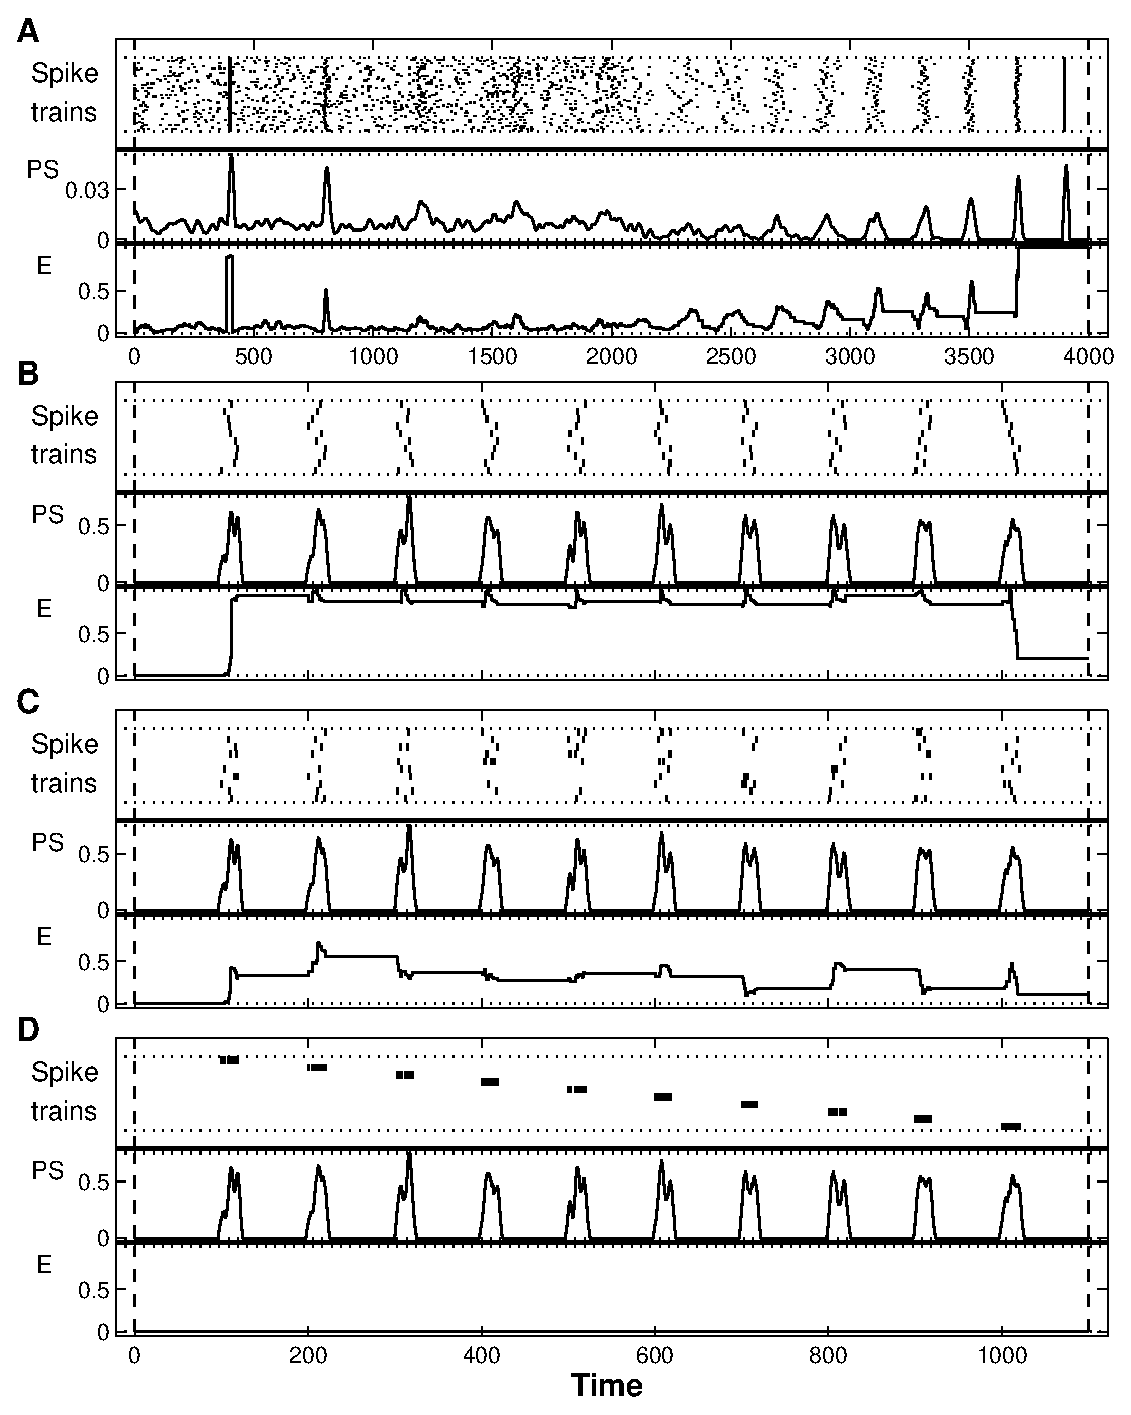
\includegraphics[width=85mm]{Fig_App_PSTH_ES.eps}
    \caption{\abb\label{fig:Fig_App_PSTH_ES} Comparison of PSTH and event synchronization. \citep{QuianQuiroga02b} XXXXX}
\end{figure}



\section{\label{App-s:ISI-SPIKE-Distance} The ISI- and the SPIKE-distance}

Both the bivariate ISI- and the bivariate SPIKE-distance rely on instantaneous values in the sense that in a first step the two sequences of discrete spike times are transformed into dissimilarity profiles, $I (t)$ and $S (t)$. These dissimilarity profiles are based on three piecewise constant quantities which for each neuron $n = 1, 2$ are assigned to every time instant (see Fig. \ref{fig:Fig1-SPIKE-Illustration}). These are the time of the preceding spike
%
\begin{equation} \label{eq:Prev-Spike}
    t_{\mathrm {P}}^{(n)} (t) = \max(t_i^{(n)} | t_i^{(n)} \leq t)  \quad t_1^{(n)} \leq t \leq t_{M_n}^{(n)},
\end{equation}
%
the time of the following spike
%
\begin{equation} \label{eq:Foll-Spike}
    t_{\mathrm {F}}^{(n)} (t) = \min(t_i^{(n)} | t_i^{(n)} > t)  \quad t_1^{(n)} \leq t \leq t_{M_n}^{(n)},
\end{equation}
%
as well as the interspike interval
%
\begin{equation} \label{eq:ISI}
    x_{\mathrm {ISI}}^{(n)} (t) = t_{\mathrm {F}}^{(n)} (t) - t_{\mathrm {P}}^{(n)} (t).
\end{equation}
%
The ambiguity regarding the definition of the very first and the very last interspike interval is resolved by placing for each spike train auxiliary leading spikes at time $t = 0$ and auxiliary trailing spikes at time $t = T$ (but see also Section \ref{sss:Edge-effect}).


\subsection{\label{App-ss:ISI-Distance} The ISI-distance}

The ISI-distance, proposed as a bivariate measure in \citep{Kreuz07c} and extended to the multi-neuron case in \citep{Kreuz09}, was the first spike train distance directly defined as the temporal average of an instantaneous dissimilarity profile. This profile is calculated as the instantaneous ratio between the interspike intervals $x_{\mathrm {ISI}}^{(1)}$ and $x_{\mathrm {ISI}}^{(2)}$ (see Eq. \ref{eq:ISI} and Fig. \ref{fig:Fig1-SPIKE-Illustration}) according to:
%
\begin{equation} \label{eq:ISI-Ratio}
    I (t) = \begin{cases}
           x_{\mathrm {ISI}}^{(1)} (t) / x_{\mathrm {ISI}}^{(2)} (t) - 1 & {\rm if} ~~ x_{\mathrm {ISI}}^{(1)} (t) \leq x_{\mathrm {ISI}}^{(2)} (t) \cr
                      - (x_{\mathrm {ISI}}^{(2)} (t) / x_{\mathrm {ISI}}^{(1)} (t) -1)     & {\rm otherwise}.
                  \end{cases}
\end{equation}
%
Since the ISI-values only change at the times of spikes, the dissimilarity profile is piecewise constant (with potential discontinuities at the spikes). The ISI-ratio equals $0$ for identical ISI in the two spike trains, and approaches $-1$ and $1$, respectively, in intervals in which the first or the second spike train is much faster than the other. In order to treat both kinds of deviations equally, the temporal averaging is performed on the absolute value of the ISI-ratio:
%
\begin{equation} \label{eq:Temporal-Average}
    D_I = \frac{1}{T} \int_{t}^T dt |I (t)|.
\end{equation}


\subsection{\label{App-ss:SPIKE-Distance} The SPIKE-distance}

In contrast to the ISI-distance, the SPIKE-distance (see \citet{Kreuz11} for the original proposal and \citet{Kreuz13} for the definite version presented here) considers the exact timing of the spikes since it is extracted from differences between the spike times of the two spike trains. 
%
% #########################################################################################
% #########################################################################################
% #################################################### Figure 1 ###########################
% #########################################################################################
% #########################################################################################
%
\begin{figure}
    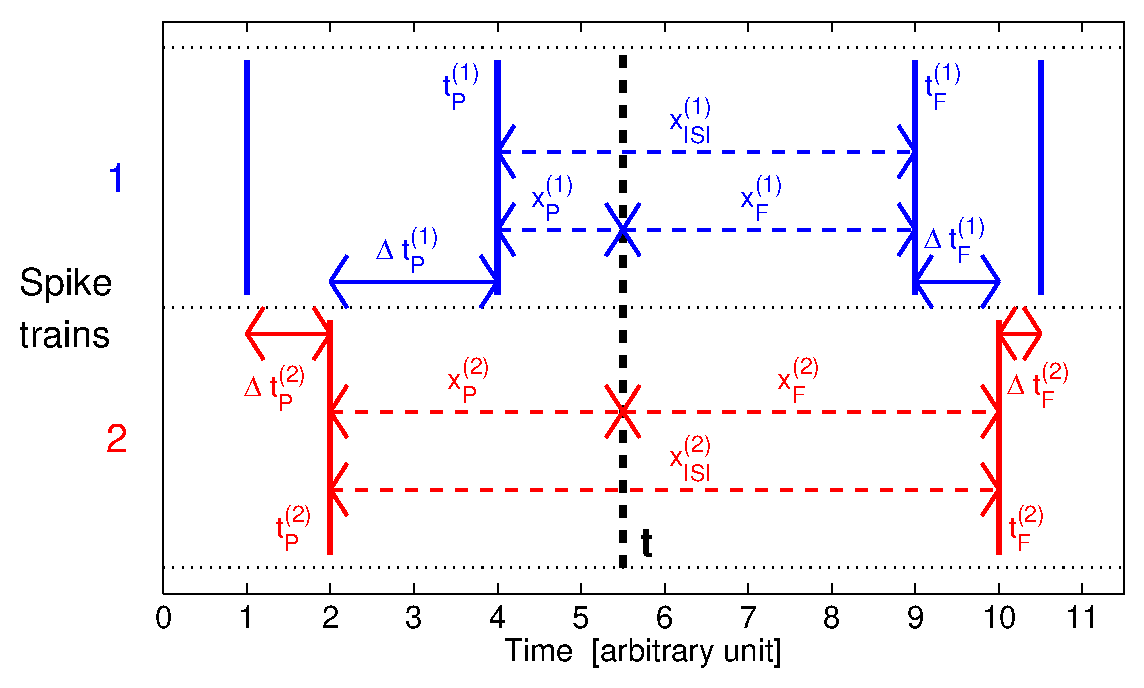
\includegraphics[width=85mm]{Fig1_SPIKE_Illustration.eps}
    \caption{\abb\label{fig:Fig1-SPIKE-Illustration} SPIKE-distance. Illustration of the local
	    quantities needed to define the dissimilarity profile $S (t)$ for an arbitrary time 
    		instant $t$.}
\end{figure}
%
% #########################################################################################
% #########################################################################################
% #################################################### Figure 1 ###########################
% #########################################################################################
% #########################################################################################

The dissimilarity profile is calculated in two steps: First for each spike the distance to the nearest spike in the other spike train is calculated, then for each time instant the relevant spike time differences are selected, weighted, and normalized. Here 'relevant' means local; each time instant is uniquely surrounded by four corner spikes: the preceding spike from the first spike train $t_{\mathrm {P}}^{(1)}$, the following spike from the first spike train $t_{\mathrm {F}}^{(1)}$, the preceding spike from the second spike train $t_{\mathrm {P}}^{(2)}$, and, finally, the following spike from the second spike train $t_{\mathrm {F}}^{(2)}$. Each of these corner spikes can be identified with a spike time difference, for example, for the previous spike of the first spike train
%
\begin{equation} \label{eq:Delta-Corner-Spike}
     \Delta t_{\mathrm {P}}^{(1)} = \min_i (| t_{\mathrm {P}}^{(1)} - t_i^{(2)} |)
\end{equation}
%
and analogously for $t_{\mathrm {F}}^{(1)}$, $t_{\mathrm {P}}^{(2)}$, and $t_{\mathrm {F}}^{(2)}$  (see Fig. \ref{fig:Fig1-SPIKE-Illustration}). For each spike train separately a locally weighted average is employed such that the differences for the closer spike dominate; the weighting factors depend on
%
\begin{equation} \label{eq:Prev-Spike-Dist}
     x_{\mathrm {P}}^{(n)} (t) = t - t_{\mathrm {P}}^{(n)} (t)
\end{equation}
%
and
%
\begin{equation} \label{eq:Foll-Spike-Dist}
     x_{\mathrm {F}}^{(n)} (t) = t_{\mathrm {F}}^{(n)} (t) - t,
\end{equation}
%
the intervals to the previous and the following spikes for each neuron $n = 1, 2$. The local weighting for the spike time differences of the first spike train reads
%
\begin{equation} \label{eq:Bi-Spike-Diss-First}
     S_1 (t) = \frac{\Delta t_{\mathrm {P}}^{(1)} x_{\mathrm {F}}^{(1)} + \Delta t_{\mathrm {F}}^{(1)} x_{\mathrm {P}}^{(1)}}{x_{\mathrm {ISI}}^{(1)}}
\end{equation}
%
and analogously $S_2 (t)$ is obtained for the second spike train. Averaging over the two spike train contributions and normalizing by the mean interspike interval yields
%
\begin{equation} \label{eq:Bi-Spike-Diss-Intermediate}
     S'' (t) = \frac{S_1 (t) + S_2 (t)}{2 \langle x_{\mathrm {ISI}}^{(n)} \rangle_n}.
\end{equation}

This quantity weights the spike time differences for each spike train according to the relative distance of the corner spike from the time instant under investigation. This way relative distances within each spike train are taken care of, while relative distances between spike trains are not. In order to get these ratios straight and to account for differences in firing rate, in a last step the two contributions from the two spike trains are locally weighted by their instantaneous interspike intervals. This leads to the definition of the dissimilarity profile
%
\begin{equation} \label{eq:Bi-Spike-Diss-Improved}
     S (t) = \frac{S_1 (t) x_{\mathrm {ISI}}^{(2)} + S_2 (t) x_{\mathrm {ISI}}^{(1)}}{2 \langle x_{\mathrm {ISI}}^{(n)} \rangle_n^2}.
\end{equation}
%
Since the dissimilarity profile is obtained from a linear interpolation of piecewise constant quantities, it is piecewise linear (with potential discontinuities at the spikes).

Similar to the ISI-distance, the SPIKE-distance is defined as the temporal average of this dissimilarity profile:
%
\begin{equation} \label{eq:Temporal-Average2}
    D_S = \frac{1}{T} \int_{t}^T dt S (t).
\end{equation}
%
The dissimilarity profile $S (t)$ and the SPIKE-distance $D_S$ as its average are bounded in the interval $[0, 1]$. The distance value $D_S = 0$ is obtained for identical spike trains only.

	
For both the ISI- and the SPIKE-distance there exists a straightforward extension to the case $N > 2$ (with $N$ denoting the number of spike trains), the averaged bivariate distance. This average over all pairs of neurons commutes with the average over time, so it is possible to achieve the same kind of time-resolved visualization as in the bivariate case by first calculating the instantaneous average $S^{\mathrm {a}} (t)$ (for the SPIKE-distance) over all pairwise instantaneous values $S^{mn} (t)$,
%
\begin{equation} \label{eq:Bivariate-Average}
    S^{\mathrm {a}} (t) = \frac{1}{N(N-1)/2}\sum_{n=1}^{N-1} \sum_{m=n+1}^N S^{mn} (t).
\end{equation}



\subsubsection{\label{App-sss:Realtime-Spike-Distance} Realtime SPIKE-distance}

The realtime SPIKE-distance $D_{S_r}$ is a modification of the SPIKE-distance with the key difference that the corresponding time profile $S_r(t)$ can be calculated online because it relies on past information only \footnote{For the ISI-distance no such causal realtime extension is possible, since it relies on the instantaneous ISI-values and thus requires knowledge about the following spikes.}. From the perspective of an online measure, the information provided by the following spikes, both their position and the length of the interspike interval, is not yet available. Like the regular (improved) SPIKE-distance $D_S$, this causal variant is also based on local spike time differences but now only two corner spikes are available, and the spikes of comparison are restricted to past spikes, e.g., for the preceding spike of the first spike train
%
\begin{equation} \label{eq:Delta-Corner-Spike-Realtime}
     \Delta t_{\mathrm {P}}^{(1)} = \min_i (| t_{\mathrm {P}}^{(1)} - t_i^{(2)} |), t_i < t.
\end{equation}
%
Since there are no following spikes available, there is no local weighting, and since there is no interspike interval, the normalization is achieved by dividing the average corner spike difference by twice the average time interval to the preceding spikes (Eq. \ref{eq:Prev-Spike-Dist}). This yields a causal indicator of local spike train dissimilarity:
%
\begin{equation} \label{eq:Bi-Spike-Diss-RT}
    S_r (t) = \frac{ \Delta t_{\mathrm {P}}^{(1)} + \Delta t_{\mathrm {P}}^{(2)}} {4 \langle x_{\mathrm {P}}^{(n)} \rangle_n}.
\end{equation}


\subsubsection{\label{App-sss:Future-Spike-Distance} Future SPIKE-distance}

The future SPIKE-distance $D_{S_f}$ can be used in triggered temporal averaging in order to evaluate the effect of certain spikes or of certain stimuli features on future spiking. It is the inverse measure to the realtime SPIKE-distance but instead of relying on past information only it relies on future information only. Again for each time instant there are just two corner spikes and the potential nearest spikes in the other spike train are future spikes only. Thus the spike time difference for the following spike of the first spike train reads
%
\begin{equation} \label{eq:Delta-Corner-Spike-Future}
     \Delta t_{\mathrm {F}}^{(1)} = \min_i (| t_{\mathrm {F}}^{(1)} - t_i^{(2)} |), t_i > t,
\end{equation}
%
and accordingly for the following spike of the second spike train. In analogy to Eq. \ref{eq:Bi-Spike-Diss-RT}, an indicator of local spike train dissimilarity is obtained as follows:
%
\begin{equation} \label{eq:Bi-Spike-Diss-FT}
    S_f (t) = \frac{ \Delta t_{\mathrm {F}}^{(1)} + \Delta t_{\mathrm {F}}^{(2)}} {4 \langle x_{\mathrm {F}}^{(n)} \rangle_n}.
\end{equation}	


\section{\label{App-s:Improvements} Improvements in this implementation}

\subsection{\label{App-ss:Edge-effect} Correction of the edge effect for the SPIKE-distance}

In previous versions of the SPIKE-distance the ambiguity regarding the definition of the initial (final) distance to the preceding (following) spike as well as the very first and the very last interspike intervals was resolved by adding to each spike train an auxiliary leading spike at time $t = 0$ and an auxiliary trailing spike at time $t = T$. This lead to spurious synchrony at the edges where by construction the dissimilarity profile reached the zero value. Here we follow a suggestion by Conor Houghton (personal communication) and at least partly correct this edge effect. We describe the correction for the beginning of the recording, it is an analogous mirror image at the end of the recording.

We count the auxiliary spikes as normal spikes which can be nearest neighbor to other spikes. But instead of calculating their spike time distance (which is always zero) we use the spike time difference of the first real spike. For the first interspike interval we know that it is at least the distance to the first spike $t_1-t_0 = t_1$ but it could be longer. So to take the local firing rate (or its inverse) into consideration we set
%
\begin{equation} \label{eq:Corrected-First-ISI}
    x_{\mathrm {ISI}} (0) = \max ( t_1, t_2 - t_1 ).
\end{equation}
%
where we use the length of the first known interspike interval $t_2-t_1$ as an upper limit of the inverse firing rate. This way we get at least a crude estimate of how much longer the first interspike interval could be.


\subsection{\label{App-ss:Sampling} Increase of memory efficiency by avoiding sampling}

Earlier versions of the codes for calculating the ISI- and the SPIKE-distance relied on sampled dissimilarity profiles. Typically the precision was set to the sampling interval of the neuronal recording. Since the dissimilarity profile has to be calculated and stored for each pair of spike trains, this resulted, for each measure, in a matrix of order 'number of sampled time instants' $\times$ 'number of spike train pairs' (i.e., $\# (t_s) \times N(N-1)/2$). For small sampling intervals and a large number of recorded spike trains this lead to memory problems.
In SPIKY we use an optimized and more memory-efficient way of storing the data where we make use of the fact that the dissimilarity profile $I (t)$ of the ISI-distance is piecewise constant and the dissimilarity profile $S (t)$ of the SPIKE-distance is piecewise linear with each interval running from one spike of the pooled spike train to the next one. Thus for each such interval (and for each pair of spike trains) we have to store only one value for the ISI-distance and two values for the SPIKE-distance, one at the beginning and one at the end of the interval. Typically the storage space required will be much smaller than for dissimilarity profiles sampled with a reasonable precision.

For both dissimilarity profiles there are instantaneous jumps at the times of the spikes since this is where the lengths of the interspike intervals and the identity of the previous and the following spikes change abruptly. In contrast to the calculation based on sampling we get the exact result since each spike is both the previous and the next spike and there is no need anymore to 'cut the corners' of the dissimilarity profiles as had to be done for the sampled dissimilarity profiles. The dissimilarity profiles $S_r(t)$ and $S_f (t)$ of the real-time and the future SPIKE-distances are hyperbolic but for these measures the exact result can be obtained by piecewise integration over all intervals of the pooled spike train.


\end{appendix}

\vspace{1cm}

\begin{thanks}
\section{\label{s:Acknowledgement} \textbf{Acknowledgements}}

NB and TK acknowledge funding support from the European Commission through the Marie Curie Initial Training Network 'Neural Engineering Transformative Technologies (NETT)', project 289146. TK also acknowledges the Italian Ministry of Foreign Affairs regarding the activity of the Joint Italian-Israeli Laboratory on Neuroscience.

TK thanks Marcus Kaiser for hosting him at the University of Newcastle, UK.
     
We thank Ralph Andrzejak, Emily Caporello, Daniel Chicharro, Tim Gentner, Conor Houghton, Jutta Kretzberg, Stefano Luccioli, Florian Mormann, Leon Paz, Friederice Pirschel, Alessandro Torcini, Jonathan Victor, and Sid Visser for useful discussions.

We also thank Thomas Alderson, Black Square, Mayte Bonilla Quintana, Hamid Charkhkar, Didier Desaintjan, Mario DiPoppa, Mahboubeh Etemadi, Marion Najac, Matthew Phillips, Eugenio Piasini, Robert Rein, Rodrigo Salazar, Michael Schaub, Eitan Schechtman, Matthew Williams, Yunguo Yu for advice and user feedback.
\end{thanks}


\begin{thebibliography}{25}

\bibitem[{Bower et al.(2012)}]{Bower12}
Bower MR, Stead M, Meyer FB, Marsh WR, Worrell GA. Spatiotemporal neuronal correlates of seizure generation in focal epilepsy. Epilepsia, 2012;53:807-16.

\bibitem[{C{Di Poppa} and Gutkin(2013)}]{DiPoppa13}
{DiPoppa} M, Gutkin BS. Correlations in background activity control persistent state stability and allow execution of working memory tasks. Front Comp Neurosci, 2013;7:139.

\bibitem[{Gruen(2009)}]{Gruen09}
Gr{\"u}n S. Data-Driven Significance Estimation for Precise Spike Correlation. J Neurophysiol, 2009;101:1126-40.

\bibitem[{Hochberg et al.(2006)}]{Hochberg06}
Hochberg LR, Serruya MD, Friehs GM, Mukand JA, Saleh M, Caplan AH, Branner A, Chen D, Penn RD, Donoghue JP. Neuronal ensemble control of prosthetic devices by a human with tetraplegia. Nature, 2006;442:164-71.

\bibitem[{Kass et al.(2005)}]{Kass05}
Kass RS, Ventura V, Brown EN. Statistical issues in the Analysis of Neuronal Data. J Neurophysiol, 2005;94:8-25.

\bibitem[{Kreuz et al.(2009)}]{Kreuz09}
Kreuz T, Chicharro D, Andrzejak RG, Haas JS, Abarbanel HDI.
  Measuring multiple spike train synchrony. J Neurosci Methods, 2009;183:287-99.

\bibitem[{Kreuz et al.(2011)}]{Kreuz11}
Kreuz T, Chicharro D, Greschner M, Andrzejak RG.
  Time-resolved and time-scale adaptive measures of spike train synchrony. J Neurosci Methods, 2011;195:92-106.

%\bibitem[{Kreuz(2011)}]{Kreuz11b}
%Kreuz T. Measures of spike train synchrony. Scholarpedia, 2011;6:11934.

\bibitem[{Kreuz et al.(2013)}]{Kreuz13}
Kreuz T, Chicharro D, Houghton C, Andrzejak RG, Mormann F.
  Monitoring spike train synchrony. J Neurophysiol, 2013;109:1457.

\bibitem[{Kreuz et al.(2007)}]{Kreuz07c}
Kreuz T, Haas JS, Morelli A, Abarbanel HDI, Politi A.
  Measuring spike train synchrony. J Neurosci Methods, 2007;165:151-61.

\bibitem[{Kumar et al.(2010)}]{Kumar10}
Kumar A, Rotter S, Aertsen A. Spiking activity propagation in neuronal networks: reconciling different perspectives on neural coding. Nature Rev Neurosci, 2010;11:615-27.

\bibitem[{Louis et al.(2010)}]{Louis10}
Louis S, Gerstein GL, Gr{\"u}n S, Diesmann M. Surrogate spike train generation through dithering in operational time. Front Comp Neurosci, 2010;4:127.

\bibitem[{Mainen and Sejnowski(1995)}]{Mainen95}
Mainen Z, Sejnowski TJ. Reliability of spike timing in neocortical neurons. Science 1995;268:1503-6.

\bibitem[{Miller and Wilson(2008)}]{Miller08}
Miller EK, Wilson MA. All My Circuits: Using Multiple Electrodes to Understand Functioning Neural Networks. Neuron, 2008;60:483-8.

\bibitem[{Mormann et~al.(2007)}]{Mormann07}
Mormann F, Andrzejak RG, Elger CE, Lehnertz K. Seizure prediction: the long and winding road. Brain, 2007;130:314-33.

\bibitem[{Nirenberg and Victor(2007)}]{Nirenberg07}
Nirenberg S, Victor JD. Analyzing the activity of large populations of neurons: how tractable is the problem? Curr Opin Neurobiol 2007;17:397-400.

\bibitem[{Papoutsi et~al.(2013)}]{Papoutsi13}
Papoutsi A, Sidiropoulou K, Cutsuridis V, Poirazi P. Induction and modulation of persistent activity in a layer v pfc microcircuit model. Front Neural Circuits 2013;7:161.

\bibitem[{Pikovsky et~al.(2001)}]{Pikovsky01}
Pikovsky AS, Rosenblum MG, Kurths J. Synchronization. A universal concept in nonlinear sciences. Cambridge Univ. Press, Cambridge, UK 2001.

\bibitem[{Quian Quiroga} et~al.(2002)]{QuianQuiroga02b}
{Quian Quiroga} R, Kreuz T, Grassberger P. Event synchronization: \textsc{A} simple and fast method to measure synchronicity and time delay patterns. Phys Rev E 2002;66:041904.

\bibitem[{Ross(1997)}]{Ross97}
Ross SM. Introduction to Probability Models. Sixth edition. Academic Press, New York, USA 1997.

\bibitem[{Rusu and Florian(2014)}]{Rusu14}
Rusu CV, RV Florian. A new class of metrics for spike trains. Neural Computation, 2014;26:306-48.

\bibitem[{Secr and Sepulchre(2014)}]{Secr14}
Sacr P, Sepulchre R. Sensitivity analysis of oscillator models in the space of phase-response curves: Oscillators as open systems. Control Systems, IEEE 2014;34:50–74.

\bibitem[{Sanchez(2008)}]{Sanchez08}
Sanchez JC, Principe JC, Nishida T, Bashirullah R, Harris JG, Fortes JAB. Technology and Signal Processing for Brain-Machine Interfaces. IEEE Signal Processing, 2008;25:29-40.

\bibitem[{Shlens et al.(2008)}]{Shlens08}
Shlens J, Rieke F, Chichilnisky EJ. Synchronized firing in the retina. Curr Opin Neurobiol, 2008;18:396-402.

\bibitem[{Thibeault et al.(2014)}]{Thibeault14}
Thibeault CM, {O'Brien} MJ, Srinivasa N. Analyzing large-scale spiking neural data with HRLAnalysis. Front. Neuroinform., 2014;8:17.

\bibitem[{Tiesinga et al.(2008)}]{Tiesinga08}
Tiesinga PHE, Fellous JM, Sejnowski TJ. Regulation of spike timing in visual cortical circuits. Nature Reviews Neuroscience 2008;9:97-107.

\bibitem[{Truccolo et al.(2011)}]{Truccolo11}
Truccolo W, Donoghue JP, Hochberg LR, Eskandar EN, Madsen JR, Anderson WS, Brown EN, Halgren E, Cash SS. Single-neuron dynamics in human focal epilepsy. Nature Neurosci, 2011;14:635-41.

\bibitem[{Victor(2005)}]{Victor05}
Victor JD. Spike train metrics. Current Opinion in Neurobiology 2005;15:585-592.

\end{thebibliography}

\bibliographystyle{elsart-harv}



%\bibliography{Kreuz_Bibliography}

%\bibliographystyle{jabbrv_plain}
%\bibliographystyle{jneurophysiol}
%\bibliographystyle{plainnat}

\end{document}
